\documentclass[../../../main.tex]{subfiles}
\begin{document}
Il peut être intéressant de stocker des éléments selon un ordre et de vouloir très rapidement trouver le minimum ou le maximum de ces éléments selon l'ordre choisi. Quelques exemples sont donnés pour montrer l'intérêt d'une structure spécialisé pour cette opération. 

\textbf{Exemple (\textit{context-switching}) :} dans un système d'exploitation, les tâches sont exécutés en alternance pour simuler leur exécution parallèle. On veut sélectionner des tâches 
\begin{itemize}
	\item qui depuis longtemps n'ont pas été traités
	\item qui sont demandantes en ressources
\end{itemize}
On peut associer à chaque tâche une pondération de chaque critère qui correspond à sa \textit{priorité}. On veut alors à chaque changement de tâche sélectionner celle de plus haute priorité. Comme le changement de tâche en lui-même doit consommer très peu de ressources, on veut une structure de données efficace, donc spécialisé pour ce but.

\textbf{Exemple (algorithmes gloutons) :} de nombreux algorithmes cherchent à optimiser numériquement des solutions en cherchant d'abord un optimum local dans l'espace des solutions. Si les différents choix sont organisés selon une file de priorité, la sélection de l'optimum local est très rapide et accélère grandement l'algorithme. C'est ce qu'on retrouve dans l'algorithme de \textit{Dijkstra} pour la recherche d'un plus court chemin dans un graphe.
\subsection{Signature}
\textbf{Première remarque :} il suffit de définir une structure de donnée permettant de trouver rapidement le minimum des élémeents. En effet, il suffit juste d'inverser la relation d'ordre pour obtenir une structure permettant de trouver rapidement le maximum des éléments.

\textit{Element} désigne un type de donnée sur lequel est défini une relation d'ordre totale\footnote{Partielle suffit en soi d'après le théorème de Szpilrajn.}

\textit{FilePriorite} utilise \textit{Booleen}, \textit{Element}
\begin{itemize}
	\item $file\_vide()\rightarrow FilePriorite$ renvoie une file de priorité sans éléments
	\item $est\_vide(FilePriorite:f)\rightarrow Booleen$ teste si la file $f$ est vide.
	\item $minimum(FilePriorite:f)\rightarrow Element$ renvoie l'élément minimal de la file de priorité
	\item $supprimer\_min(FilePriorite:f)\rightarrow FilePriorite$ renvoie $f$ dont on a retiré l'élément minimal
	\item $inserer(FilePriorite:f, Element:x)\rightarrow FilePriorite$ renvoie $f$ à laquelle on a ajouté l'élément $x$
\end{itemize}
On construit la routine de commodité $extraire\_min(\text{mut }FilePriorite:f)\rightarrow Element$ qui renvoie l'élément minimal de $f$ et le supprime de $f$.

On implanter les files de priorité par des arbres AVLs. Les complexités temporelles des routines $minimum$ $supprimer\_min$ et $inserer$ sont alors des fonctions de $O(log_2(n))$, où $n$ est le nombre d'éléments dans la file de priorité.

On présente ici une autre implantation plus efficace et bien plus simple à mettre en oeuvre, le \textit{tas minimum}.
\subsection{Arbres complets}
Les tas minimums sont forment un cas particulier d'arbres presque complets. On définit donc d'abord cette notion et comment on peut implanter très facilement et très efficacement des arbres presque complets.
\subsubsection{Principe}
\definition{Arbres presque complets} {
	L'ensemble $A^p_X$ des \textit{arbres presque complets} sur un ensemble ordonné $(X, \leq)$ est défini par induction par :
	$$\left\{\begin{array}{cll}
	\mathcal{B} & : & E\in A^p_X \\
	\mathcal{I} & : & \forall g, d\in A^p_X, \forall x\in X, (0 \leq h(g) - h(d) \leq 1) \Rightarrow (g, x, d)\in A^p_X
\end{array}\right.$$
	En français : pour tout sous-arbre $(g, x, d)$ d'un arbre,
	\begin{itemize}
		\item le sous-arbre gauche est toujours plus haut que le sous-arbre droit
		\item le sous-arbre est équilibré
	\end{itemize}
}
\textbf{Exemple :} on représente ci-dessous les 9 premiers arbres presque complets :

\begin{minipage}{0.2\textwidth}
\begin{center}
	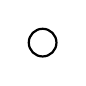
\begin{tikzpicture}[node distance={5mm}, thick, main/.style = {draw, circle, minimum size=1em}] 
	% Sommets :
	\node[main] (0) {}; 
	% Arêtes
	\end{tikzpicture} 
\end{center}
\end{minipage}
\begin{minipage}{0.2\textwidth}
\begin{center}
	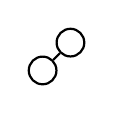
\begin{tikzpicture}[node distance={5mm}, thick, main/.style = {draw, circle, minimum size=1em}] 
	% Sommets :
	\node[main] (0) {}; 
	\node[main] (1) [below left of=0] {};
	% Arêtes
	\draw (0) -- (1);
	\end{tikzpicture} 
\end{center}
\end{minipage}
\begin{minipage}{0.2\textwidth}
\begin{center}
	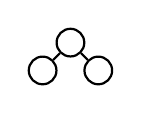
\begin{tikzpicture}[node distance={5mm}, thick, main/.style = {draw, circle, minimum size=1em}] 
	% Sommets :
	\node[main] (0) {}; 
	\node[main] (1) [below left of=0] {};
	\node[main] (2) [below right of=0] {};
	% Arêtes
	\draw (0) -- (1);
	\draw (0) -- (2);
	\end{tikzpicture} 
\end{center}
\end{minipage}
\begin{minipage}{0.2\textwidth}
\begin{center}
	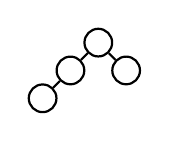
\begin{tikzpicture}[node distance={5mm}, thick, main/.style = {draw, circle, minimum size=1em}] 
	% Sommets :
	\node[main] (0) {}; 
	\node[main] (1) [below left of=0] {};
	\node[main] (2) [below right of=0] {};
	\node[main] (3) [below left of=1] {};
	% Arêtes
	\draw (0) -- (1);
	\draw (0) -- (2);
	\draw (1) -- (3);
	\end{tikzpicture} 
\end{center}
\end{minipage}
\begin{minipage}{0.2\textwidth}
\begin{center}
	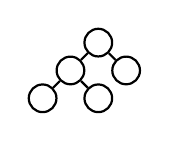
\begin{tikzpicture}[node distance={5mm}, thick, main/.style = {draw, circle, minimum size=1em}] 
	% Sommets :
	\node[main] (0) {}; 
	\node[main] (1) [below left of=0] {};
	\node[main] (2) [below right of=0] {};
	\node[main] (3) [below left of=1] {};
	\node[main] (4) [below right of=1] {};
	% Arêtes
	\draw (0) -- (1);
	\draw (0) -- (2);
	\draw (1) -- (3);
	\draw (1) -- (4);
	\end{tikzpicture} 
\end{center}
\end{minipage}

\begin{minipage}{0.25\textwidth}
\begin{center}
	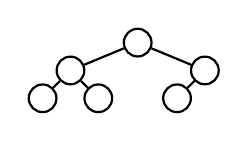
\begin{tikzpicture}[node distance={5mm}, thick, main/.style = {draw, circle, minimum size=1em}] 
	% Sommets :
	\node[main] (0) {}; 
	\node[main] (1) [below left of=0, xshift=-5mm] {};
	\node[main] (2) [below right of=0, xshift=5mm] {};
	\node[main] (3) [below left of=1] {};
	\node[main] (4) [below right of=1] {};
	\node[main] (5) [below left of=2] {};
	% Arêtes
	\draw (0) -- (1);
	\draw (0) -- (2);
	\draw (1) -- (3);
	\draw (1) -- (4);
	\draw (2) -- (5);
	\end{tikzpicture} 
\end{center}
\end{minipage}
\begin{minipage}{0.25\textwidth}
\begin{center}
	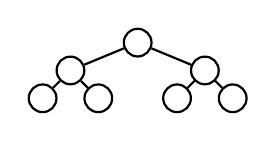
\begin{tikzpicture}[node distance={5mm}, thick, main/.style = {draw, circle, minimum size=1em}] 
	% Sommets :
	\node[main] (0) {}; 
	\node[main] (1) [below left of=0, xshift=-5mm] {};
	\node[main] (2) [below right of=0, xshift=5mm] {};
	\node[main] (3) [below left of=1] {};
	\node[main] (4) [below right of=1] {};
	\node[main] (5) [below left of=2] {};
	\node[main] (6) [below right of=2] {};
	% Arêtes
	\draw (0) -- (1);
	\draw (0) -- (2);
	\draw (1) -- (3);
	\draw (1) -- (4);
	\draw (2) -- (5);
	\draw (2) -- (6);
	\end{tikzpicture} 
\end{center}
\end{minipage}
\begin{minipage}{0.25\textwidth}
\begin{center}
	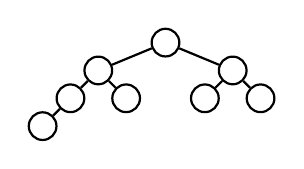
\begin{tikzpicture}[node distance={5mm}, thick, main/.style = {draw, circle, minimum size=1em}] 
	% Sommets :
	\node[main] (0) {}; 
	\node[main] (1) [below left of=0, xshift=-5mm] {};
	\node[main] (2) [below right of=0, xshift=5mm] {};
	\node[main] (3) [below left of=1] {};
	\node[main] (4) [below right of=1] {};
	\node[main] (5) [below left of=2] {};
	\node[main] (6) [below right of=2] {};
	\node[main] (7) [below left of=3] {};
	% Arêtes
	\draw (0) -- (1);
	\draw (0) -- (2);
	\draw (1) -- (3);
	\draw (1) -- (4);
	\draw (2) -- (5);
	\draw (2) -- (6);
	\draw (3) -- (7);
	\end{tikzpicture} 
\end{center}
\end{minipage}
\begin{minipage}{0.25\textwidth}
\begin{center}
	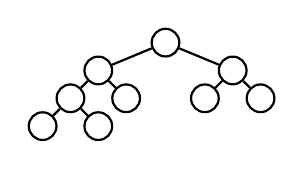
\begin{tikzpicture}[node distance={5mm}, thick, main/.style = {draw, circle, minimum size=1em}] 
	% Sommets :
	\node[main] (0) {}; 
	\node[main] (1) [below left of=0, xshift=-5mm] {};
	\node[main] (2) [below right of=0, xshift=5mm] {};
	\node[main] (3) [below left of=1] {};
	\node[main] (4) [below right of=1] {};
	\node[main] (5) [below left of=2] {};
	\node[main] (6) [below right of=2] {};
	\node[main] (7) [below left of=3] {};
	\node[main] (8) [below right of=3] {};
	% Arêtes
	\draw (0) -- (1);
	\draw (0) -- (2);
	\draw (1) -- (3);
	\draw (1) -- (4);
	\draw (2) -- (5);
	\draw (2) -- (6);
	\draw (3) -- (7);
	\draw (3) -- (8);
	\end{tikzpicture} 
\end{center}
\end{minipage}
\begin{center}
\captionof{figure}{les 9 premiers arbres presque complets\label{fig:arbres_presque_complets}}
\end{center}
\subsubsection{Implantation par tableau}
\subsection{Tas minimum}
On décrit ici une implantation efficace des files de priorité grâce à la structure de donnée de \textit{Tas minimum}.

\definition{Arbre de tournoi} {
	L'ensemble $A^t_X$ des \textit{arbres tournoi} sur un ensemble ordonné $(X, \leq)$ est défini par induction par :
	$$\left\{\begin{array}{cll}
	\mathcal{B} & : & E\in A^t_X \\
	\mathcal{I} & : & \forall g, d\in A^t_X, \forall x\in X, \left[(\forall{n_{l}\in{elts(g)}}, x \leq n_{l}) \wedge (\forall{n_{r}}\in{elts(d)}, x \leq n_r)\right] \Rightarrow (g, x, d)\in A^t_X
\end{array}\right.$$
	En français : la racine d'un arbre tournoi est plus petite que tous les éléments des sous-arbres gauche et droit.
}
\textbf{Exemple :} avec $X = \mathbb{Z}$
\begin{center}
	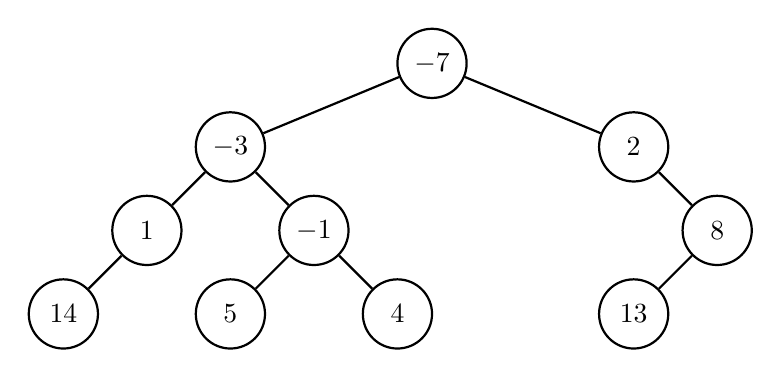
\begin{tikzpicture}[node distance={15mm}, thick, main/.style = {draw, circle, minimum size=2.5em}] 
	% Sommets :
	\node[main] (0) {$-7$}; 
	\node[main] (1) [below left of=0, xshift=-15mm] {$-3$};
	\node[main] (2) [below right of=0, xshift=15mm] {$2$};
	\node[main] (3) [below left of=1] {$1$};
	\node[main] (4) [below right of=1] {$-1$};
	\node[main] (5) [below left of=4] {$5$};
	\node[main] (7) [below right of=4] {$4$};
	\node[main] (6) [below right of=2] {$8$};
	\node[main] (8) [below left of=6] {$13$};
	\node[main] (9) [below left of=3] {$14$};
	% Arêtes
	\draw (0) -- (1);
	\draw (0) -- (2);
	\draw (1) -- (3);
	\draw (1) -- (4);
	\draw (4) -- (5);
	\draw (2) -- (6);
	\draw (7) -- (4);
	\draw (8) -- (6);
	\draw (9) -- (3);
	\end{tikzpicture} 
	\captionof{figure}{Un arbre tournoi\label{fig:abre_tournoi}}
\end{center}
\proposition{Croissance des chemins} Un arbre binaire est un arbre tournoi \textit{si et seulement si} tous les chemins de la racine aux feuilles sont croissants.

\textbf{Démonstration :} par induction, découle immédiatement de la définition

\definition{Tas} {
	Un \textit{tas} est un arbre de tournoi presque complets.
}
\subsection{Exercices}
\end{document}